\documentclass{article}

\usepackage[margin=1in]{geometry}
\usepackage{amsmath}
\usepackage{amsfonts}
\usepackage{graphicx}
\usepackage{float}
\usepackage{listings}
\usepackage{color}


\definecolor{mygreen}{RGB}{28,172,0} % color values Red, Green, Blue
\definecolor{mylilas}{RGB}{170,55,241}

\lstset{language=Matlab,%
    %basicstyle=\color{red},
    breaklines=true,%
    morekeywords={matlab2tikz},
    keywordstyle=\color{blue},%
    morekeywords=[2]{1}, keywordstyle=[2]{\color{black}},
    identifierstyle=\color{black},%
    stringstyle=\color{mylilas},
    commentstyle=\color{mygreen},%
    showstringspaces=false,%without this there will be a symbol in the places where there is a space
    numbers=left,%
    numberstyle={\tiny \color{black}},% size of the numbers
    numbersep=9pt, % this defines how far the numbers are from the text
    emph=[1]{for,end,break},emphstyle=[1]\color{red}, %some words to emphasise
    %emph=[2]{word1,word2}, emphstyle=[2]{style},    
}


\title{Homework 1: Digital Control (ECEN 5458)}
\author{Zachary Vogel}
\date{\today}

\newcommand{\rank}{\text{rank}}

\begin{document}
\maketitle

\section*{Problem 1}
This question asks us to do problem 1.1 in the book.
\subsection*{(a)}
First it asks for the sampling rate, in Hertz, of the range signal plotted on the radar screen?\\
At six revolutions a minute, the antenna makes a full rotation once very ten seconds. Thus the sampling rate of the screen must be $0.1$Hz.

\subsection*{(b)}
Now the question asks for the sampling rate, in Hertz, of the controller's instructions?\\
First, convert miles per hour to miles per second:
\[540/3600=0.15\]
miles per second. There is supposed to be an update ever nine miles. Thus, we need to send an instruction every 60 seconds. That means the instruction rate is $1/60$ Hz.

\subsection*{(c)}
This part asks whether or not the following signals are discrete, digital or analog:
\begin{itemize}
    \item Aircraft's Range from the Airport: Analog
    \item The range data plotted on the radar screen: Discrete
    \item Controllers' Instructions to Pilot: Digital
    \item Pilot's actions on the aircraft control surfaces: Analog
\end{itemize}

\subsection*{(d)}
Then, the problem asks if this is a continuous, sampled-data, or digital control system?\\
I believe it is a digital control system because it contains a digital part in the instructions to the pilot.

\subsection*{(e)}
Here, we are asked if it is possible for the radar to see a straight line, when in reality the plane is flying in a zig zag. This is pretty easy to see. As long as the zig zag pattern has a period equal to $P_{\text{zigzag}}=\frac{P_{\text{radar}}}{2^n}$ for $n=0,1,\dots,\infty$ and the direction of net movement of the zigzag is towards the radar. The lowest frequency necessary for the radar to see a straight line would be the frequency that the radar samples at.


\section*{Problem 2}
This problem gives a closed loop system and asks several questions about the system. The system has a feedback gain of 1 and two transfer functions, $D(s)$ and $G(s)$ making up the controller and plant. These transfer functions are:
\[D(s)=K\cfrac{s+a}{s+b}\quad G(s)=\cfrac{1}{s(s+c)}\]
\subsection*{(a)}
First the problem asks for the closed loop transfer function of the system. This is just:
\[U(s)=\cfrac{Y(s)}{R(s)}=\cfrac{D(s)G(s)}{1+D(s)G(s)}=\cfrac{K\cfrac{s+a}{s(s+b)(s+c)}}{1+K\cfrac{s+a}{s(s+b)(s+c)}}=\cfrac{K(s+a)}{s(s+b)(s+c)+K(s+a)}\]
\[U(s)=\cfrac{K(s+a)}{s^3+s^2(c+b)+s(K+bc)+a}\]

\subsection*{(b)}
Given $K=2$, $a=1$, $b=2$, and $c=3$. Determine the closed-loop poles and zeros. Then determine if the system is stable. To do this we need to factor the Denominator of our transfer function.
\[U(s)=\cfrac{2(s+1)}{s^3+5s^2+12s+1}=\cfrac{2(s+1)}{(s+0.086392)(s+2.45681-2.35364j)(s+2.45681+2.35364j)}\]
Here we see that all of our poles are in the left half plane. Therefore, the system is stable.

\subsection*{(c)}
This problem asks me to use the Final Value Theorem to determine the steady-state value of $y(t)$ given:
\[r(t)=u(t)=\left \{\begin{array}{ll}0, & t<0\\1, & t\geq 0\end{array}\right .\]
First, we need the Laplace Transform of $r(t)$, which is $R(s)=\frac{1}{s}$. Then, the Final Value theorem states that:
\[\begin{array}{c}\lim_{t\to\infty}y(t)=\lim_{s\to 0}sU(s)R(s)=\cfrac{2s+2}{s^3+5s^2+12s+1}\\=\cfrac{2}{1}=2\end{array}\]

\section*{Problem 3}
Note: Just going to answer the questinos instead of being verbose.\\

The results of teh siso design do agree with my answer from part 2b. The poles and zeros are different by a small amount.\\

The final value does not agree with 2c for me. Wondering what I did wrong.\\

Both plots are attached to this document.

\section*{Problem 4}
Problem 3.1\\
\subsection*{(a)}
Here we are asked to design a lead compensator for the plant $G(s)=\frac{1}{s^2}$ such that the complex poles are at $s=-4.4\pm 4.4j$.\\
To do this, we recognize the form of a lead compensator:
\[D(s)=\cfrac{s+a}{s+b}\quad b>a\]
Then the transfer function is:
\[\cfrac{DG}{1+DG}=\cfrac{s+a}{s^3+bs^2+s+a}\]
Set the denominator equal to:
\[s^3+bs^2+s+a=(s+c)(s+4.4+4.4j)(s+4.4-4.4j)\]
Then do long division to get that:
\[s^2+(b-c)s+(1-bc+c^2)=s^2+8.8s+38.72\]
and
\[c*(1-bc+c^2)=a\]
Solving these three equations yields:
\[b=4.5136,\quad a=-165.9708,\quad c=-4.2864\]
This yields the desired complex poles.
\subsection*{(b)}
Now the problem wants us to consider a $T/2$ delay defined by:
\[G_h(s)=\cfrac{\frac{2}{T}}{s+\frac{2}{T}}\]
with sample rates of $\omega_s=5$Hz, $10$Hz, and $20$Hz. With these it wants us to find the revised root locations. This is when I move to Matlab. The code is in the Appendix, the values can be seen in the table below:
\begin{table}[H]
    \centering
    \begin{tabular}{l|l|l|l|l|}
        \hline
        Frequency & New Pole & Complex pole 1 & Complex pole 2 & old pole\\\hline
        5Hz& -11.7688&-3.2578+5.1757j &-3.2578-5.1757j &3.7707 \\\hline
        10Hz& -20.5508&-3.9745+4.9722j &-3.9745-4.9722j &3.9863 \\\hline
        20Hz&-40.1436 &-4.2460+4.7002j &-4.2460-4.7002j &4.1220 \\\hline
    \end{tabular}
\end{table}

\subsection*{(c)}
My closed loop system is unstable for all T because you never asked me to design a stable system, just one with the correct poles. The complex poles never pass into the right half plane though. Below is a plot of the desired locus.
\begin{figure}[H]
    \centering
    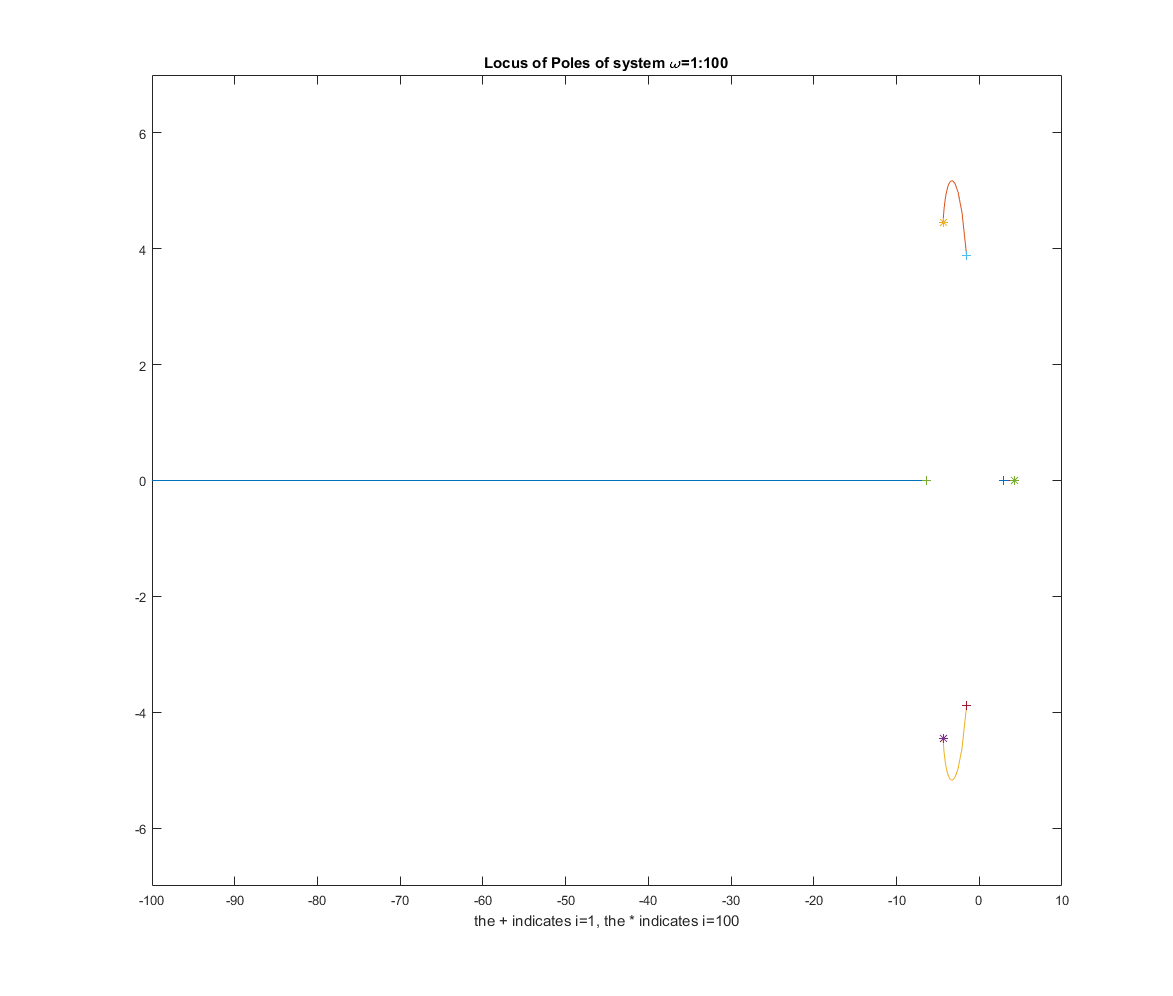
\includegraphics[width=\textwidth]{HW1_P4c.png}
\end{figure}

\subsection*{(d)}
Given:
\[\mathcal{L}(u(t))=U(s)\]
show that
\[\mathcal{L}(u(t-\frac{T}{2}))=e^{-\frac{sT}{2}}U(s)\]
Here we go
\[\int_0^\infty u(t-\frac{T}{2})e^{-st}dt\]
substitute in $r=t-\frac{T}{2}$ to get:
\[\int_0^\infty u(r)e^{-s(r+\frac{T}{2})}dr=e^{-\frac{sT}{2}}\int_0^\infty u(r)e^{-sr}dr=e^{-\frac{sT}{2}}U(s)\]

\subsection*{(e)}
My answer is the same as in part C unfortunately. Didn't have time to go back through and do the analysis again. Sorry, won't happen next time. All the bode plots are in the Appendix, the code for this whole problem is in the other appendix.


\section*{Problem 5}
Problem 3.2: This problem asks us to redo example 3.1 using the backward euler approximation instead of the forward one.\\
Starting with the Transfer function:
\[D(s)=\cfrac{U(s)}{E(s)}=K_o\cfrac{s+a}{s+b}\]
this corresponds to the differential equation:
\[\dot{u}+bu=K_0(\dot{e}+ae)\]
Turning it into a difference equation with the approximation $\dot{u}=\frac{u(k)-u(k-1)}{T}$ we get:
\[\cfrac{u(k)-u(k-1)}{T}+bu(k)=K_o\cfrac{e(k)-e(k-1)}{T}+K_oae(k)\]
reorganizing terms we get:
\[u_k=\cfrac{K_o(e_k(aT+1)-e_{k-1})+u_{k-1}}{1+bT}\]
Now set $K_o=70$, $a=2$, and $b=10$. The coefficients of interest are $c_0=\frac{1}{1+10T}$, $c_1=\frac{-70}{1+10T}$ and $c_2=\frac{70(1+2T)}{(1+10T)}$. For $T=1$, $c_0=\frac{1}{11}$, $c_1=\frac{-70}{11}$, and $c_2=\frac{210}{11}$. For $T=\frac{1}{100}$, $c_0\approx 1$, $c_1\approx -70$, and $c_2\approx 70$.

\section*{Problem 6}
Problem 4.2:
\subsection*{(a)}
Here we are deriving the area under the curve of the parabola defined by the points $e_k, e_{k-1}, e_{k-2}$. We want to take the area between the points $t=T(k-1)$ and $t=Tk$.\\
To begin, realize what we want is:
\[u_k=u_{k-1}+\int_{T(k-1)}^{Tk} ax^2+bx+c dx\]
Where a, b and c are determined by $e_k,$ $e_{k-1}$, $e_{k-2}$. To do this, we will be using a divided difference method. The form of our parabola is:
\[e(x)=a_0+a_1(x-x_0)+a_2(x-x_0)(x-x_1)\]
where $x_0=(k-2)T$, $x_1=(k-1)T$ and $x_2=kT$. The we evaluate at a few points:
\[e(x_0)=a_0=e_{k-2}\]
\[e(x_1)=e_{k-1}=a_0+a_1(x_1-x_0)\implies a_1=\cfrac{e_{k-1}-e_{k-2}}{T}\]
\[e(x_2)=e_k=a_0+a_1(x_2-x_0)+a_2(x_2-x_0)(x_2-x_1)\implies a_2=\cfrac{e_k-2e_{k-1}+e_{k-2}}{2T^2}\]
Now to integrate each part from $x_1$ to $x_2$
\[\int_{x_1}^{x_2}e_{k-2}dx=e_{k-2}T\]
\[\int_{x_1}^{x_2}\cfrac{e_{k-1}-e_{k-2}}{T}(x-x_0)dx=\cfrac{e_{k-1}-e_{k-2}}{T}\left (\cfrac{3}{2}T^2\right )=\cfrac{3}{2}(e_{k-1}-e_{k-2})T\]
\[\begin{array}{c}\int_{x_1}^{x_2}a_2(x-x_0)(x-x_1)dx=a_2 \left (\cfrac{x^3}{3}-\cfrac{(x_0+x_1)x^2}{2}+x_0x_1x\right )\bigg |_{x_1}^{x_2}\\
=\cfrac{T^3}{3}-\cfrac{3}{2}T^3+2T^3=\cfrac{5T^3}{6}\end{array}\]
Note that there is some algebra missing here. If you want that as well, I guess I can type it up. The final result is then:
\[\int_{x_1}^{x_2}e(x)dx=T\left (-\cfrac{1}{12}e_{k-2}+\cfrac{7}{6}e_{k-1}+\cfrac{5}{12}e_k\right )\]

\subsection*{(b)}
Now find the transfer function of the derived discrete time system and determine where the poles and zeros are.\\
Writing it out we have:
\[u_k=u_{k-1}+T\left (-\cfrac{1}{12}e_{k-2}+\cfrac{7}{6}e_{k-1}+\cfrac{5}{12}e_k\right )\]
This transforms to:
\[U(z)=U(z)z^{-1}+TE(z)\left (-\cfrac{z^{-2}}{12}+\cfrac{7z^{-1}}{6}+\cfrac{5}{12}\right )\]
\[H(z)=\frac{U(z)}{E(z)}=\cfrac{T(-z^{-1}+14+5z)}{12(z-1)}\]
This isn't ideal for plotting poles and zeros so instead I will do that for $\frac{1}{H(z)}$:
\[\frac{1}{H(z)}=\cfrac{12 (z^2-z)}{T(5z^2+14z-1)}\]
\begin{figure}[H]
    \centering
    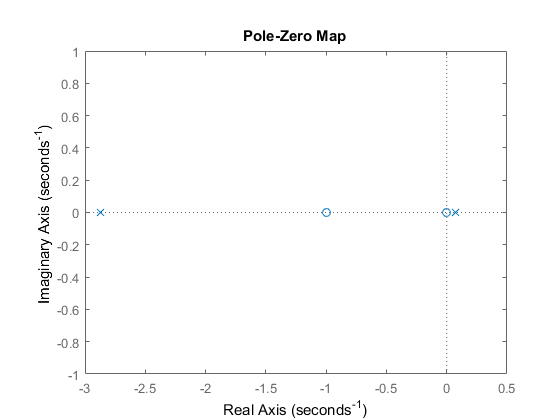
\includegraphics[width=0.7\textwidth]{HW1_6b.png}
    \caption{pole zero map of $\frac{1}{H(z)}$}
\end{figure}

\section*{Problem 7}
Problem 4.13(a) Here we define the one-sided Z-transform as:
\[F(z)=\sum_{k=0}^\infty f(k)z^{-k}\]
The problem asks us to show that the Z-transform of $f(k+1)$ is:
\[\mathcal{Z}(f(k+1))=zF(z)-zf(0)\]
To begin, let us write out the system:
\[\sum_{k=0}^\infty f(k+1)z^{-k}\]
now make the substitution $m=k+1$:
\[=\sum_{m=1}^\infty f(m)z^{-m+1}\]
Then we use some basic algebra:
\[=z\sum_{m=1}^\infty f(m)z^{-m}=z\left (\sum_{k=0}^\infty f(k)z^{-k}-f(0)\right )=zF(z)-zf(0)\]

\section*{Problem 8}
Problem 4.20 The problem gives us a discrete transfer function with a region of convergence for $\lvert z\rvert >2$.:
\[U(z)=\cfrac{z}{(z-1)(z-2)}\]
\subsection*{(a)}
Using the final value theorem, we can find the final value for the system.
\[\lim_{z\to 1}(z-1)\cfrac{z}{(z-1)(z-2)}=\cfrac{1}{1-2}=-1\]

\subsection*{(b)}
One can check this by taking the inverse Z-transform and evaluating at $k=\infty$:
\[U(z)=\cfrac{z}{(z-1)(z-2)}=\cfrac{-1}{z-1}+\cfrac{2}{z-2}\]
\[\mathcal{Z}^{-1}(U(z))=-1^{n-1}u(k-1)+2*2^{k-1}u(k-1)=(-1+2^k)u(k-1)\]
\[u(k\to\infty)=\infty\]

\subsection*{(c)}
Why is there a discrepancy?\\
The discrepancy is caused by the convergence region being $\lvert z\rvert>2$. Since we have a pole at $z=2$, that is not removed when using the final value theorem, the problem fails. If we multiply by $z-2$ instead of $z-1$ we get the correct answer.

\section*{Problem 9}
My partner is Kaitlyn Garifi. We are going to work on the tape disc controller for more accurate positioning of the laser reader, to increase density of tape disc memory.

\appendix
\section{Bode Plots 4e}
No sampling
\begin{figure}[H]
    \centering
    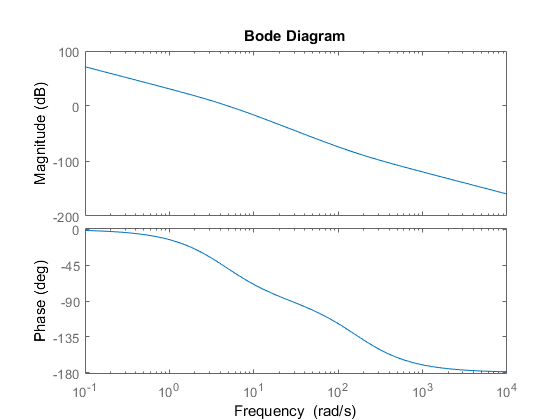
\includegraphics[width=0.7\textwidth]{P4e1.png}
\end{figure}
1 Hz
\begin{figure}[H]
    \centering
    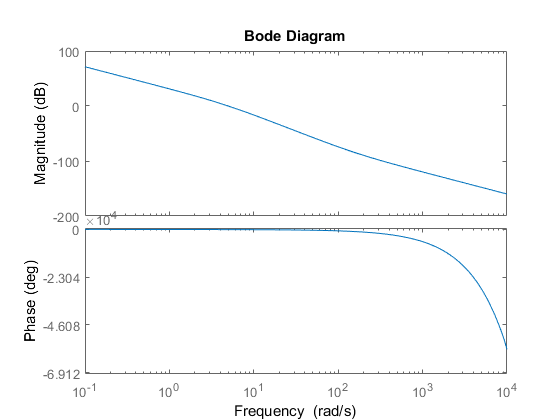
\includegraphics[width=0.7\textwidth]{P4e1hz.png}
\end{figure}
5 Hz
\begin{figure}[H]
    \centering
    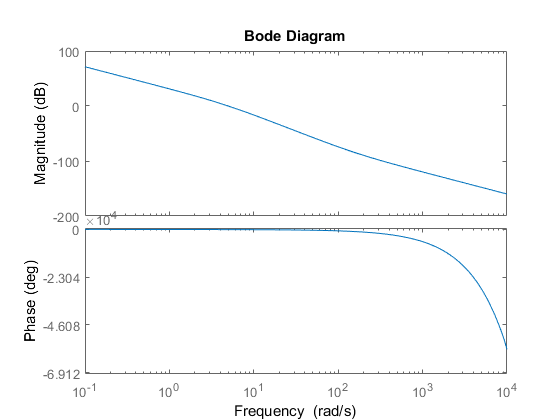
\includegraphics[width=0.7\textwidth]{P4e5hz.png}
\end{figure}
10 Hz
\begin{figure}[H]
    \centering
    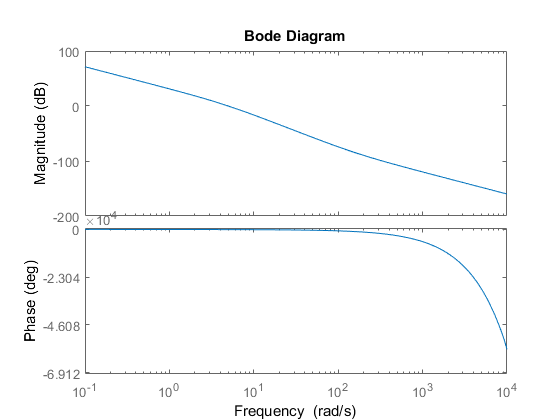
\includegraphics[width=0.7\textwidth]{P4e10hz.png}
\end{figure}
15 Hz
\begin{figure}[H]
    \centering
    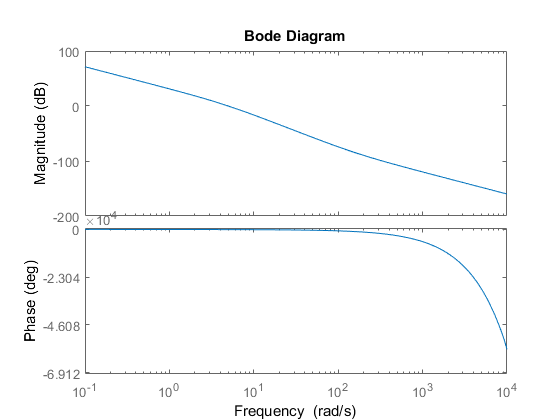
\includegraphics[width=0.7\textwidth]{P4e15hz.png}
\end{figure}
20 Hz
\begin{figure}[H]
    \centering
    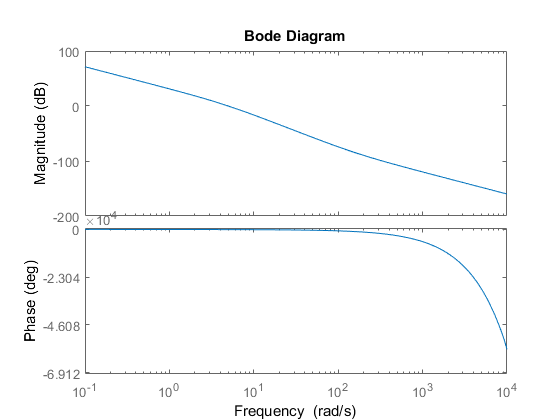
\includegraphics[width=0.7\textwidth]{P4e20hz.png}
\end{figure}
\section{Code}
\lstinputlisting{HW1_P4.m}


\end{document}
